% the code below specifies where the figures are stored
\ifpdf
    \graphicspath{{preliminary_neutral_islands/figures/PNG/}{example_chapter/figures/PDF/}{preliminary_neutral_islands/figures/}}
\else
    \graphicspath{{preliminary_neutral_islands/figures/EPS/}{preliminary_neutral_islands/figures/}}
\fi


\chapter{Preliminary Stacking Results}\label{sec:Preliminary}

In this chapter we briefly present preliminary results obtained from applying the stacking methods described in \S \ref{sec:NeutralIslands} to spectra provided to us by Andrei Mesinger, Ian McGreer, and Valentina D'Odorico. These spectra are described in \citet{McGreer:2014qwa},\footnote{Technically, we use all of the spectra in \citet{McGreer:2014qwa} except for J0002+2550 and MMT observations of J1137+3549. This detail is reflected in Table \ref{tab:speclist}.} with the basic properties shown in their Table 1. We have recreated their table here (Table \ref{tab:speclist}) for convenience. 


% Description of spectra provided to us by McGreer, Mesinger, and D'Odorico. Worth remembering that we actually only have _most_ of these...
\begin{table}
 \begin{center}
 \caption{Quasar spectra\label{tab:speclist}}
 \begin{tabular}{lrrrrl}
 \hline
 Object & $z$ & $z_{\rm AB}$ & $t_{\rm exp}$ (hr) & $\langle\tau_{\rm eff,lim}^\alpha\rangle$ & source \\
 \hline
J1420-1602 &    5.73 &   19.7 &    4.00 &    5.3 & MagE \\
J0927+2001 &    5.77 &   19.9 &    0.33 &    3.8 & ESI \\
J1044-0125 &    5.78 &   19.2 &    4.79 &    5.2 & MagE \\
J0836+0054 &    5.81 &   18.7 &    0.33 &    4.7 & ESI \\
           &         &        &    4.00 &    3.9 & MMT \\
           &         &        &    2.27 &    5.9 & XShooter \\
%J0002+2550 &    5.82 &   19.0 &    2.76 &    3.6 & MMT \\
J0840+5624 &    5.84 &   19.8 &    0.33 &    4.1 & ESI \\
J1335+3533 &    5.90 &   20.1 &    0.33 &    3.8 & ESI \\
J1411+1217 &    5.90 &   19.6 &    1.00 &    3.7 & ESI \\
J0148+0600 &    5.92 &   19.4 &   10.00 &    6.3 & XShooter \\
J0841+2905 &    5.98 &   19.8 &    0.33 &    3.5 & ESI \\
J1306+0356 &    6.02 &   19.5 &    0.25 &    4.3 & ESI \\
           &         &        &   11.50 &    5.4 & XShooter \\
J0818+1722 &    6.02 &   19.6 &    4.50 &    4.6 & MMT \\
           &         &        &    5.90 &    5.7 & XShooter \\
J1137+3549 &    6.03 &   19.5 &    0.67 &    3.8 & ESI \\
%           &         &        &    2.33 &    3.7 & MMT \\
J2054-0005 &    6.04 &   20.7 &   11.00 &    4.4 & MagE \\
J0353+0104 &    6.05 &   20.5 &    1.00 &    3.5 & ESI \\
J1630+4012 &    6.07 &   20.4 &    4.39 &    3.2 & MMT \\
J0842+1218 &    6.08 &   19.6 &    0.67 &    4.0 & ESI \\
J1509-1749 &    6.12 &   20.3 &    6.00 &    4.7 & MagE \\
           &         &        &    8.32 &    5.2 & XShooter \\
J1319+0950 &    6.13 &   20.0 &   10.00 &    5.7 & XShooter \\
J1623+3112 &    6.25 &   20.1 &    1.00 &    4.2 & ESI \\
J1030+0524 &    6.31 &   20.0 &   10.32 &    5.3 & ESI \\
           &         &        &    7.46 &    5.4 & XShooter \\
J1148+5251 &    6.42 &   20.1 &   11.00 &    6.0 & ESI \\
 \hline
 \end{tabular}
 \end{center}
 Note: $\langle\tau_{\rm eff,lim}^\alpha\rangle$ is the median effective optical depth in
       the \lya\ forest for a pixel (binned to 3.3 cMpc) with a flux equivalent to the $1\sigma$
       noise estimate.
\end{table}


When working with actual spectra, there are a few details that we must deal with which we did not need to discuss while using mock spectra. Specifically, the actual spectra have varying spectral resolutions, varying signal-to-noise values, do not have periodic boundary conditions, and are not at a fixed redshift. We deal with the differing spectra resolutions by smoothing all spectra with a Gaussian kernel with full width at half max equal to 50 km/s and resampling them at this resolution. We deal with the varying signal-to-noise values by incorporating an inverse-variance weighting scheme when averaging transmission in different regions of different spectra. Typically, when implementing an inverse-weighting scheme, the ``variance'' is the noise variance. However, in our case we have two effective sources of noise: noise in the spectra themselves and resonant absorption throughout the spectra. In other words, if we are trying to measure an underlying damping wing signal, then additional resonant absorption occurring in the span of the damping wing is effectively a source of noise for us. To incorporate this, we perform the inverse-variance weighting using a variance $\sigma_{\text{tot}}^{2}$ defined by 

\begin{align}
\sigma_{\text{tot}}^{2} &\equiv \sigma_{\text{N}}^{2} + \sigma_{\text{F}}^{2}
\end{align}

where $\sigma_{\text{N}}^{2}$ is the spectrum's noise variance and $\sigma_{\text{F}}^{2}$ is the variance in the flux of the spectra due to actual absorption, calculated after smoothing all spectra to a common resolution and after binning in redshift. Thus, each region of transmission incorporated into the stack is weighted by the $1/\sigma_{\text{tot}}^{2}$ value associated with that spectrum. 

To accommodate the fact that the spectra evolve in redshift along the line of sight, we perform stacking in two discrete redshift bins, one incorporating $5.5 \leq z_{\text{gap}} \leq 5.7$ and one with $5.7 \leq z_{\text{gap}} \leq 6$, where $z_{\text{gap}}$ is the redshift of the dark gap that we are stacking at the boundaries of. To incorporate the fact that the spectra do not have periodic boundary conditions, we require that regions of transmission extend for at least $\Delta v_{\text{min}} = 5000\kms$ before terminating at the end of the spectrum. This is to prevent somewhat artificial noise in the stacked transmission resulting from regions of transmission that encountered the edge of the spectral coverage before spanning the entire velocity range of the stack. 


With the exceptions of these caveats, though, we perform the stacking in the same qualitative manner as described thus far. Namely, when searching for the HI damping wing, we stack \lya\ transmission outside of dark gaps in the \lyb\ forest and set the minimum length of a ``large'' dark gap to be $L_{\text{min}} = 300\kms$ and the maximum length of a ``small'' dark gap to be $L_{\text{max}} = 300\kms$ \textit{in \lyb}. These precise values differ somewhat from those used earlier in order to increase statistics. Based on the signal-to-noise values, number, and spectral resolution of the spectra in Table \ref{tab:speclist}, we do not expect to be able to detect absorption due to deuterium. However, we perform the search anyway and stack \lyb\ transmission outside of any dark gaps \textit{in \lyb} whose length are at least $L_{\text{min}} = 100\kms$. 


In \Fig{fig:LargePreliminaryLowZ} and \Fig{fig:LargePreliminary}, we show the preliminary \lya\ stacking results for the low-$z$ and high-$z$ bins, respectively. In each figure, the top panel shows the results of stacking outside of small dark gaps while the bottom panel shows the results of stacking outside of large dark gaps. In each case, the solid lines are for mock spectra generated to roughly mimic the spectral resolution and signal-to-noise characteristics of the true spectra.\footnote{The model spectra used here actually result in a mean flux that is \textit{smaller} than we get when stacking spectra from Table \ref{tab:speclist}. We apply a scaling factor to the mock spectra's stacked flux in order for the two to match. We have generated mock spectra with a range of $\langle F \rangle \lesssim 0.1$ and find that this approximation is appropriate.} The colors match those in earlier plots, namely, $\axhi = 0$ (magenta), 0.05 (cyan), 0.22 (blue), and 0.35 (black). The stacked transmission for the spectra in Table \ref{tab:speclist} is shown in dashed green.


There are two comparisons that we can make here. First, we can compare the stacked transmission outside of large and small dark gaps to the simulated stacked transmission under different neutral fractions. For this comparison, let us first focus on stacked transmission outside of small dark gaps. For both redshift bins, the stacked appears relatively noisy and not well-fit by any of the simulated curves. While the stacked transmission in this case appears larger for $\Delta v > 3000\kms$ than for $\Delta v < 3000\kms$, the behavior is not consistent with our expectations for that from damping-wing absorption. Specifically, we would expect the smallest stacked transmission to occur for very small velocity separations, as can be seen in the simulated stacked transmission outside of the large dark gaps. However, in dashed-green curve, there is a spike in stacked transmission for velocity separations of less than a few hundred km/s. It is unclear if this excess absorption is a genuine feature or simply the result of statistical fluctuations. One possibility is that, if absorption systems are clustered, the excess absorption could be akin to the ``2-halo'' term described in Appendix C. 


\begin{figure}[!ht]
  \centering
  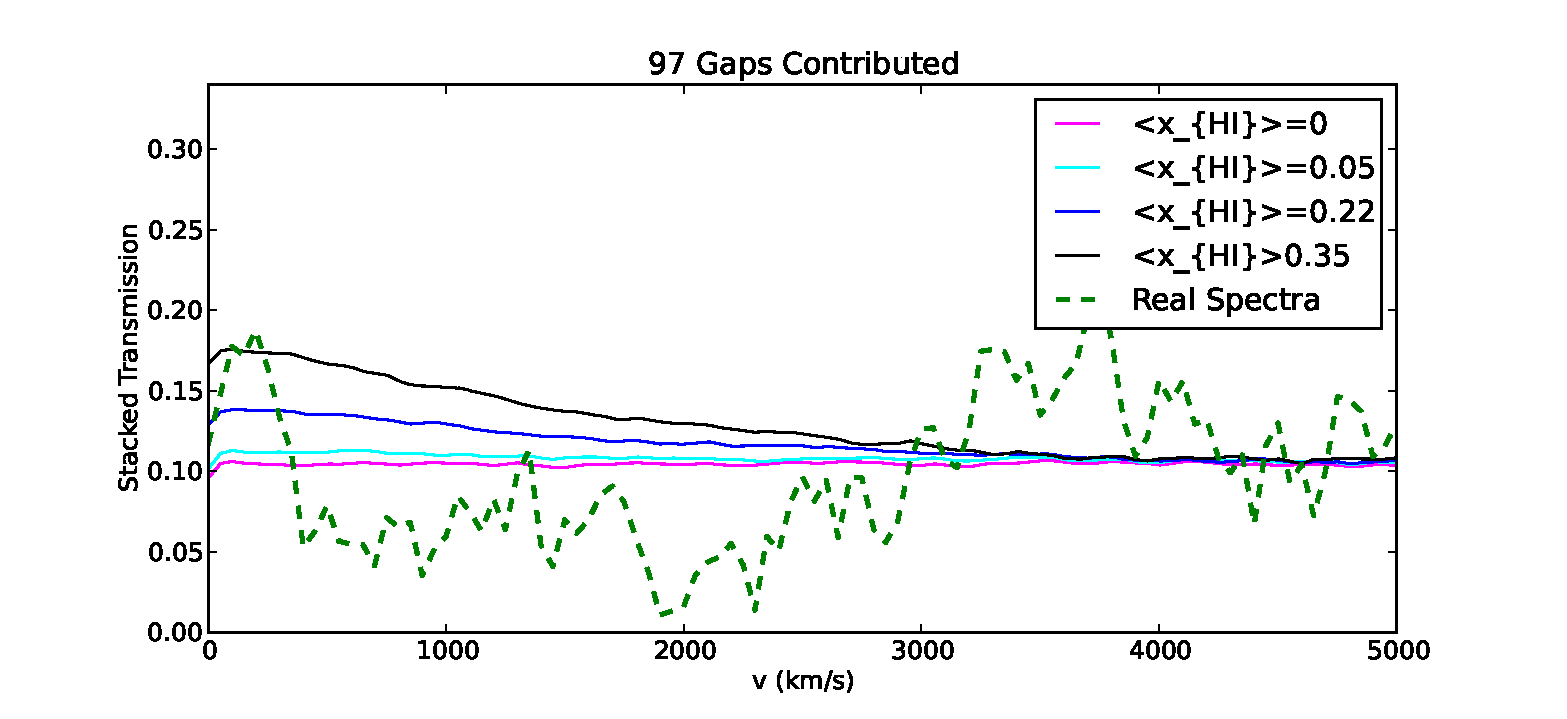
\includegraphics[width=12cm]{smallstack_lowz_mesinger.eps}
  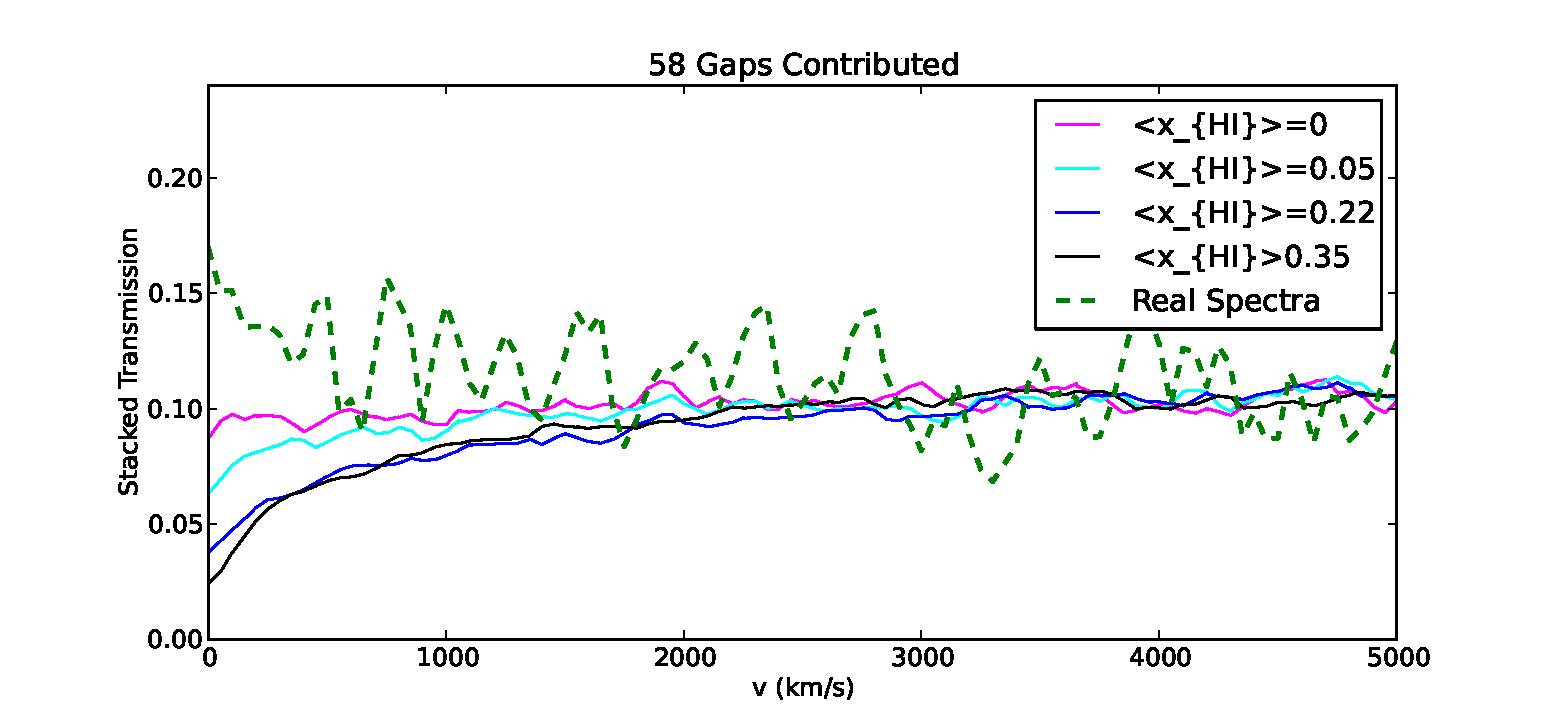
\includegraphics[width=12cm]{largestack_lowz_mesinger.eps}
  \caption{The above figure shows the results of stacking \lya\ transmission outside of dark gaps in the \lyb\ portion of the spectrum with $L < 300\kms$ (top) and $L > 300\kms$ (bottom) for dark gaps with $5.5 \leq z_{\text{gap}} \leq 5.7$. The solid curves are generated using mock spectra assuming $\axhi = 0$ (magenta), 0.05 (cyan), 0.22 (blue), and 0.35 (black). The dashed green line shows the stacking results for the spectra described in Table \ref{tab:speclist}.}
  \label{fig:LargePreliminaryLowZ}
\end{figure}

\begin{figure}[!ht]
  \centering
  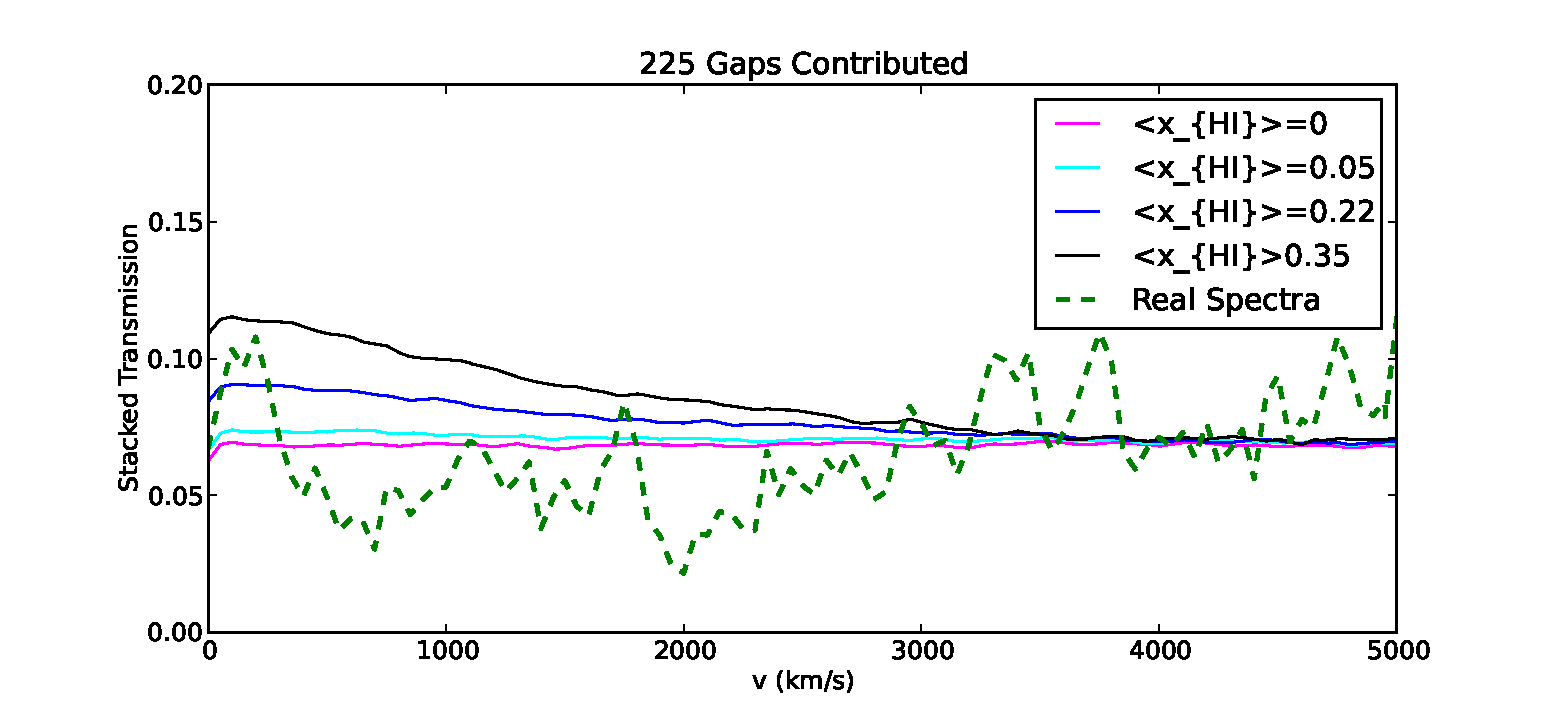
\includegraphics[width=12cm]{smallstack_mesinger.eps}
  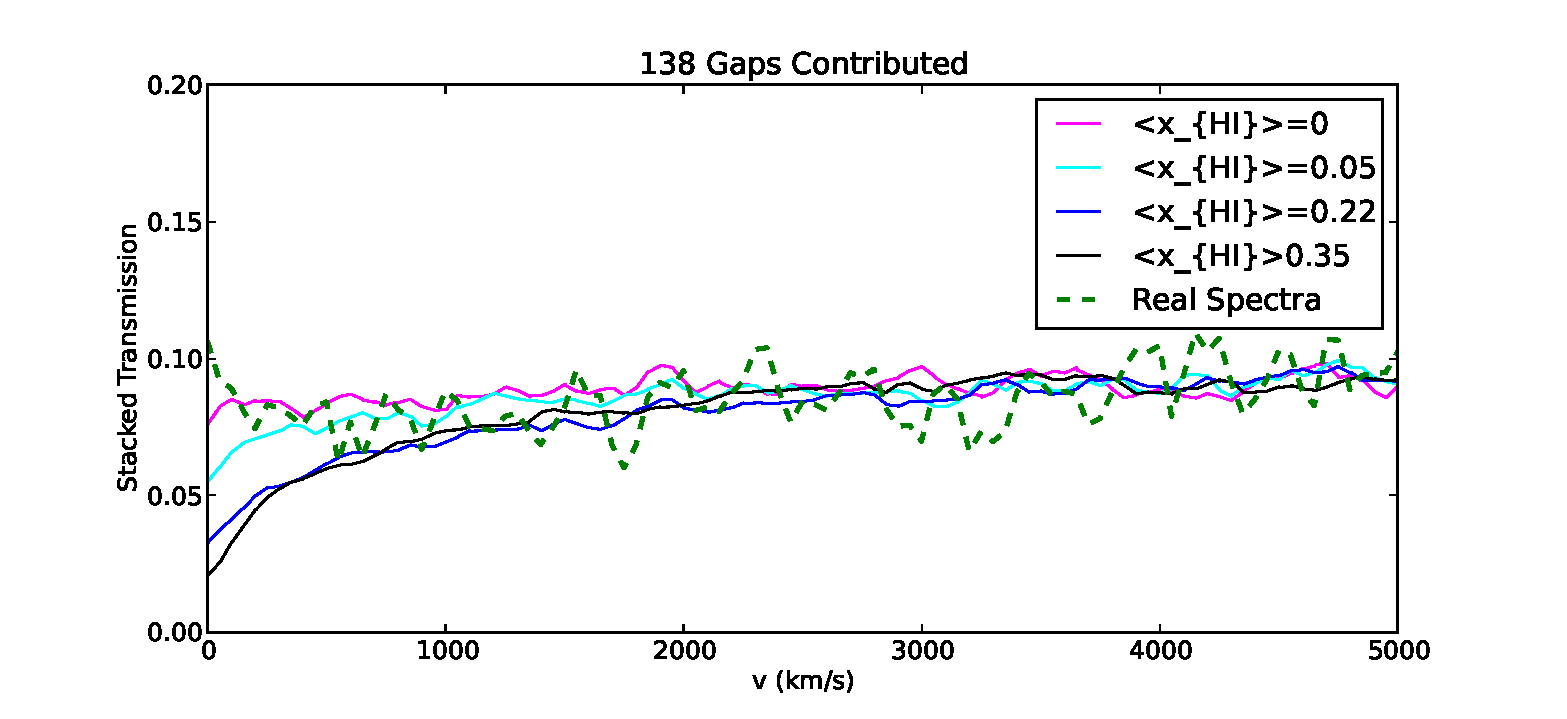
\includegraphics[width=12cm]{largestack_mesinger.eps}
  \caption{This figure is identical to \Fig{fig:LargePreliminaryLowZ} except we stack outside of dark gaps with $5.7 \leq z_{\text{gap}} \leq 6$.}
  \label{fig:LargePreliminary}
\end{figure}


The stacked transmission outside of large dark gaps in both the low-$z$ and high-$z$ bins appear less noisy. In the lower redshift bin, the stacked transmission is relatively flat but starts off large and falls toward the mean transmission by $\Delta v \approx 3000\kms$. This behavior is not precisely the same as for the mock spectra but does not show any excess absorption that can be attributed to the damping wing. Meanwhile, in the high-$z$ bin, the stacked transmission is much flatter. While the stacked transmission shows a slight increase over the course of $\Delta v \sim 500-5000\kms$, the transmission is initially rather high -- not suggestive of damping-wing absorption. If the stacked transmission from the mock spectra is reliable, this curve is consistent with a neutral fraction of $\axhi \lesssim 0.05$. However, since the analogous curve for the low-$z$ bin did not match well with the model curves, this comparison is likely risky. 


These comparisons have the disadvantage that they rely on simulations and are therefore somewhat model-dependent. Earlier in this chapter we proposed directly comparing the stacked transmission outside of large and small dark gaps as a test for the damping wing. If damping-wing absorption was significant, we would expect the associated absorbers to result in large dark gaps, such that stacked transmission outside of large dark gaps would show significant excess absorption to that outside of small dark gaps. Performing this comparison by eye for the top/bottom panels of \Fig{fig:LargePreliminaryLowZ} and \Fig{fig:LargePreliminary}, we see the opposite behavior: stacked transmission outside of \textit{small} dark gaps shows more absorption than that outside of large dark gaps. While we do not have an explanation for this behavior, it is not suggestive of a damping wing.


Lastly, in \Fig{fig:dcheck} and \Fig{fig:dcheck_lowz} we compare the stacked \lyb\ transmission redward (blue) and blueward (green) of dark gaps in the \lyb\ forest with $L_{\text{gap}} > 100\kms$. We should emphasize that, due to the number and quality of the spectra used, we do not expect to observe excess absorption due to deuterium, even for a significantly-neutral IGM. However, we perform the test anyway and find that the stacked redward and blueward transmission agree very well. 


Therefore, while we have not performed a rigorous statistical analysis of the stacked transmission using these spectra, after a preliminary look we do not see any obvious evidence of neutral hydrogen at $z < 6$. We emphasize, however, that this is by no means conclusive evidence that reionization has completed by this time. 

\begin{figure}[!ht]
  \centering
  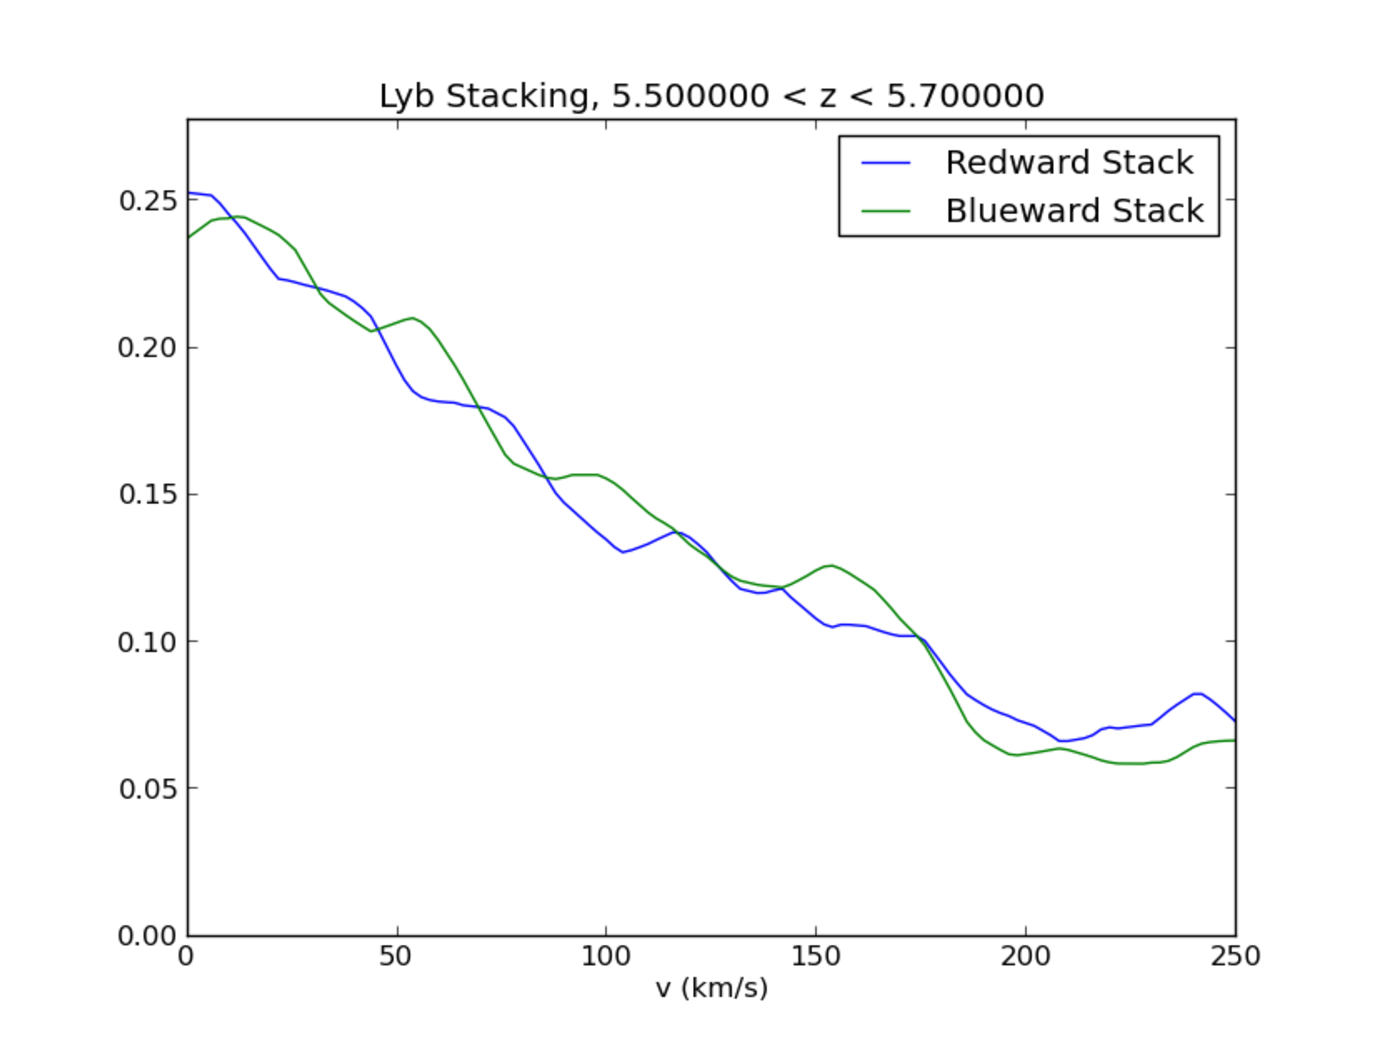
\includegraphics[width=8cm]{Lyb_lowz.eps}
  \caption{This figure shows the results of stacking \lyb\ transmission outside of dark gaps with $L > 100\kms$ in the spectra described in Table \ref{tab:speclist}. For this figure, we stack outside of dark gaps with $5.5 \leq z_{\text{gap}} \leq 5.7$.}
  \label{fig:dcheck_lowz}
\end{figure}

\begin{figure}[!ht]
  \centering
  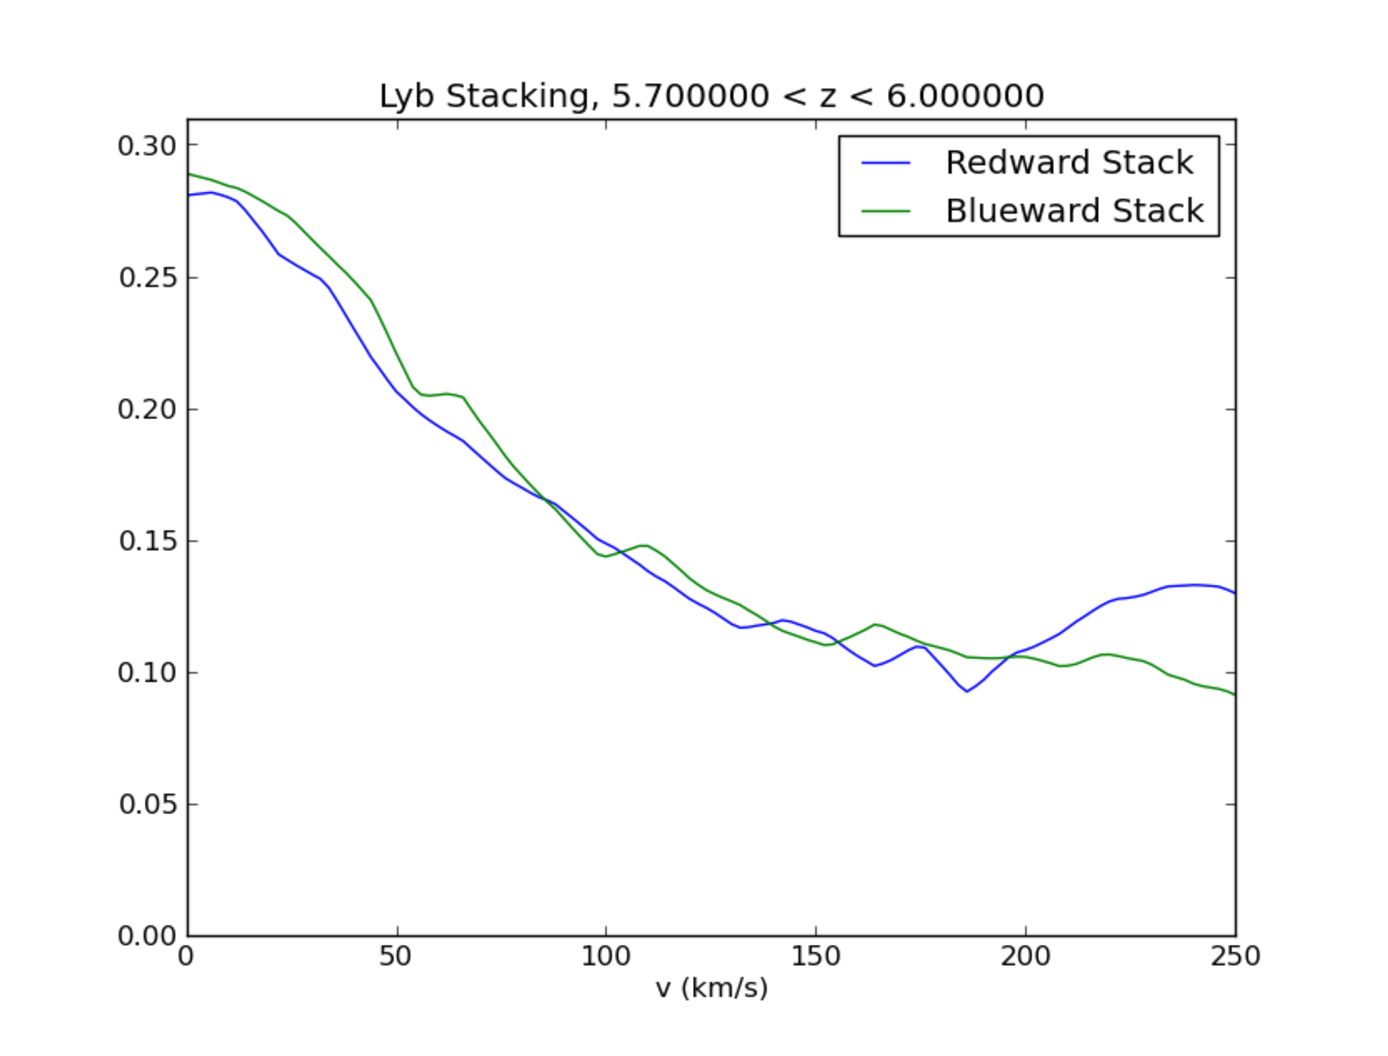
\includegraphics[width=8cm]{Lyb_highz.eps}
  \caption{This figure is identical to \Fig{fig:dcheck_lowz} except we stack outside of dark gaps with $5.7 \leq z_{\text{gap}} \leq 6$.}
  \label{fig:dcheck}
\end{figure}